%ekg_7 Zusammenfassung

\section{Zusammenfassung}

In diesem Kapitel werden die Zielsetzung und die tatsächlichen Ergebnisse mit einander verglichen. Außerdem werden Verbesserungen und Funktionen aufgeführt, die in einer möglichen zweiten Iteration des Projektes umgesetzt werden können.

\subsection{Was wurde erreicht}

Die grundlegende Aufgabenstellung war die Entwicklung eines Ein-Kanal-EKG-Gerätes für den mobilen Heimgebrauch. Diese Anforderung wurde erfüllt. Das EKG-Signal wird mittels Einmalelektroden an der Körperoberfläche gemessen, analog gefiltert und verstärkt und dann mit einer Frequenz von \SI{250}{\hertz} analog-digital gewandelt. Hierfür wurde das zu erwartende Signal analysiert und eine Filterschaltung entworfen. Zur Abtastung des Signals wurde ein Mikrocontroller der Firma TI programmiert. Dieser verarbeitet das Signal, die Benutzereingaben und verwaltet alle peripheren Module. 

Zur Anzeige des Signalverlaufs wurde ein Touch-Display programmiert, dass via UART vom Prozessor angesprochen wird. Das Display dient ebenso zur Steuerung und Information des Benutzers. Die Signalanzeige auf dem Display erfolgt in beiden Aufnahmemodi, kann jedoch weder in X- noch in Y-Richtung manuell skaliert werden. 

Zusätzlich zur Anzeige auf dem integrierten Display, wurde eine Android-App entwickelt. Die Kommunikation erfolgt zwischen EKG-Prozessor und Bluetoothmodul über UART und zwischen Bluetoothmodul und Smartphne über Bluetooth 2.0. In der App wird das Echtzeitsignal dargestellt und kann auch manuell skaliert werden. Weiterführende Kommunikation zwischen App und EKG-Gerät wurde nicht implementiert.

Die ADC-Werte werden vom Mikroprozessor über eine der SPI-Schnittstellen auf eine SD-Karte gespeichert. Hierfür wurde ein Kartentreiber auf dem Prozessor implementiert. Neben den Signal-Werten werden außerdem der Zeitpunkt der Messung, seit Beginn der Messung, sowie der ausgewählte Benutzer auf der jeweiligen CSV-Datei gespeichert. 

Wie geplant wurden zwei Aufnahmemodi implementiert. Im Kurzzeit-EKG wird das Signal auf dem Display und wahlweise zusätzlich in der App angezeigt. Außerdem wird die Herzfrequenz kontinuierlich berechnet und bei entsprechendem Anlass eine Warnmeldung über einen zu langsamen oder zu schnellen Puls angezeigt. Im Langzeit-EKG kann das Signal um Energie zu sparen nur auf dem integrierten Display angezeigt werden. Zudem wurde in dieser Aufnahme ein dedizierter Energiesparmodus implementiert, in dem der Prozessor die komplette Peripherie abschaltet und nur etwa alle \SI{4}{\sec} wieder anschaltet um die Daten auf die SD-Karte zu speichern. In diesem Modus ist eine Akkulaufzeit von 48 bis 60 Stunden möglich, prinzipiell sind also zwei Langzeitaufnahmen hintereinander ohne Aufladen möglich. 

Zur Energieversorgung aller Module werden über Aufwärtswandler und LDO zwei verschiedene Versorgungsspannungen aus der Akkuspannung generiert. Ebenso wurden Maßnahmen, wie Verpolschutz und Schmelzsicherungen, zum Schutz der Schaltung entwickelt. Um alle elektronischen Baugruppen zusammenzufügen wurde ein PCB mit dem Layouttool Altium erstellt und danach die Platine bei einem externen Hersteller gefertigt. Danach wurde die Platine von Hand bestückt und im Reflow-Ofen gelötet. 

Für das Gehäuse wurde mittels CAD-Programm ein Model erstellt, welches als Vorlage für den 3D-Druck diente. 

Nach den separaten Modultests, folgte die Integration aller Baugruppen und der Gesamttest. In Abbildung \ref{fig_EKG-Gerät} ist das fertige EKG-Gerät mit Elektrodenkabel abgebildet.

\begin{figure} [!h]
	%\centering
	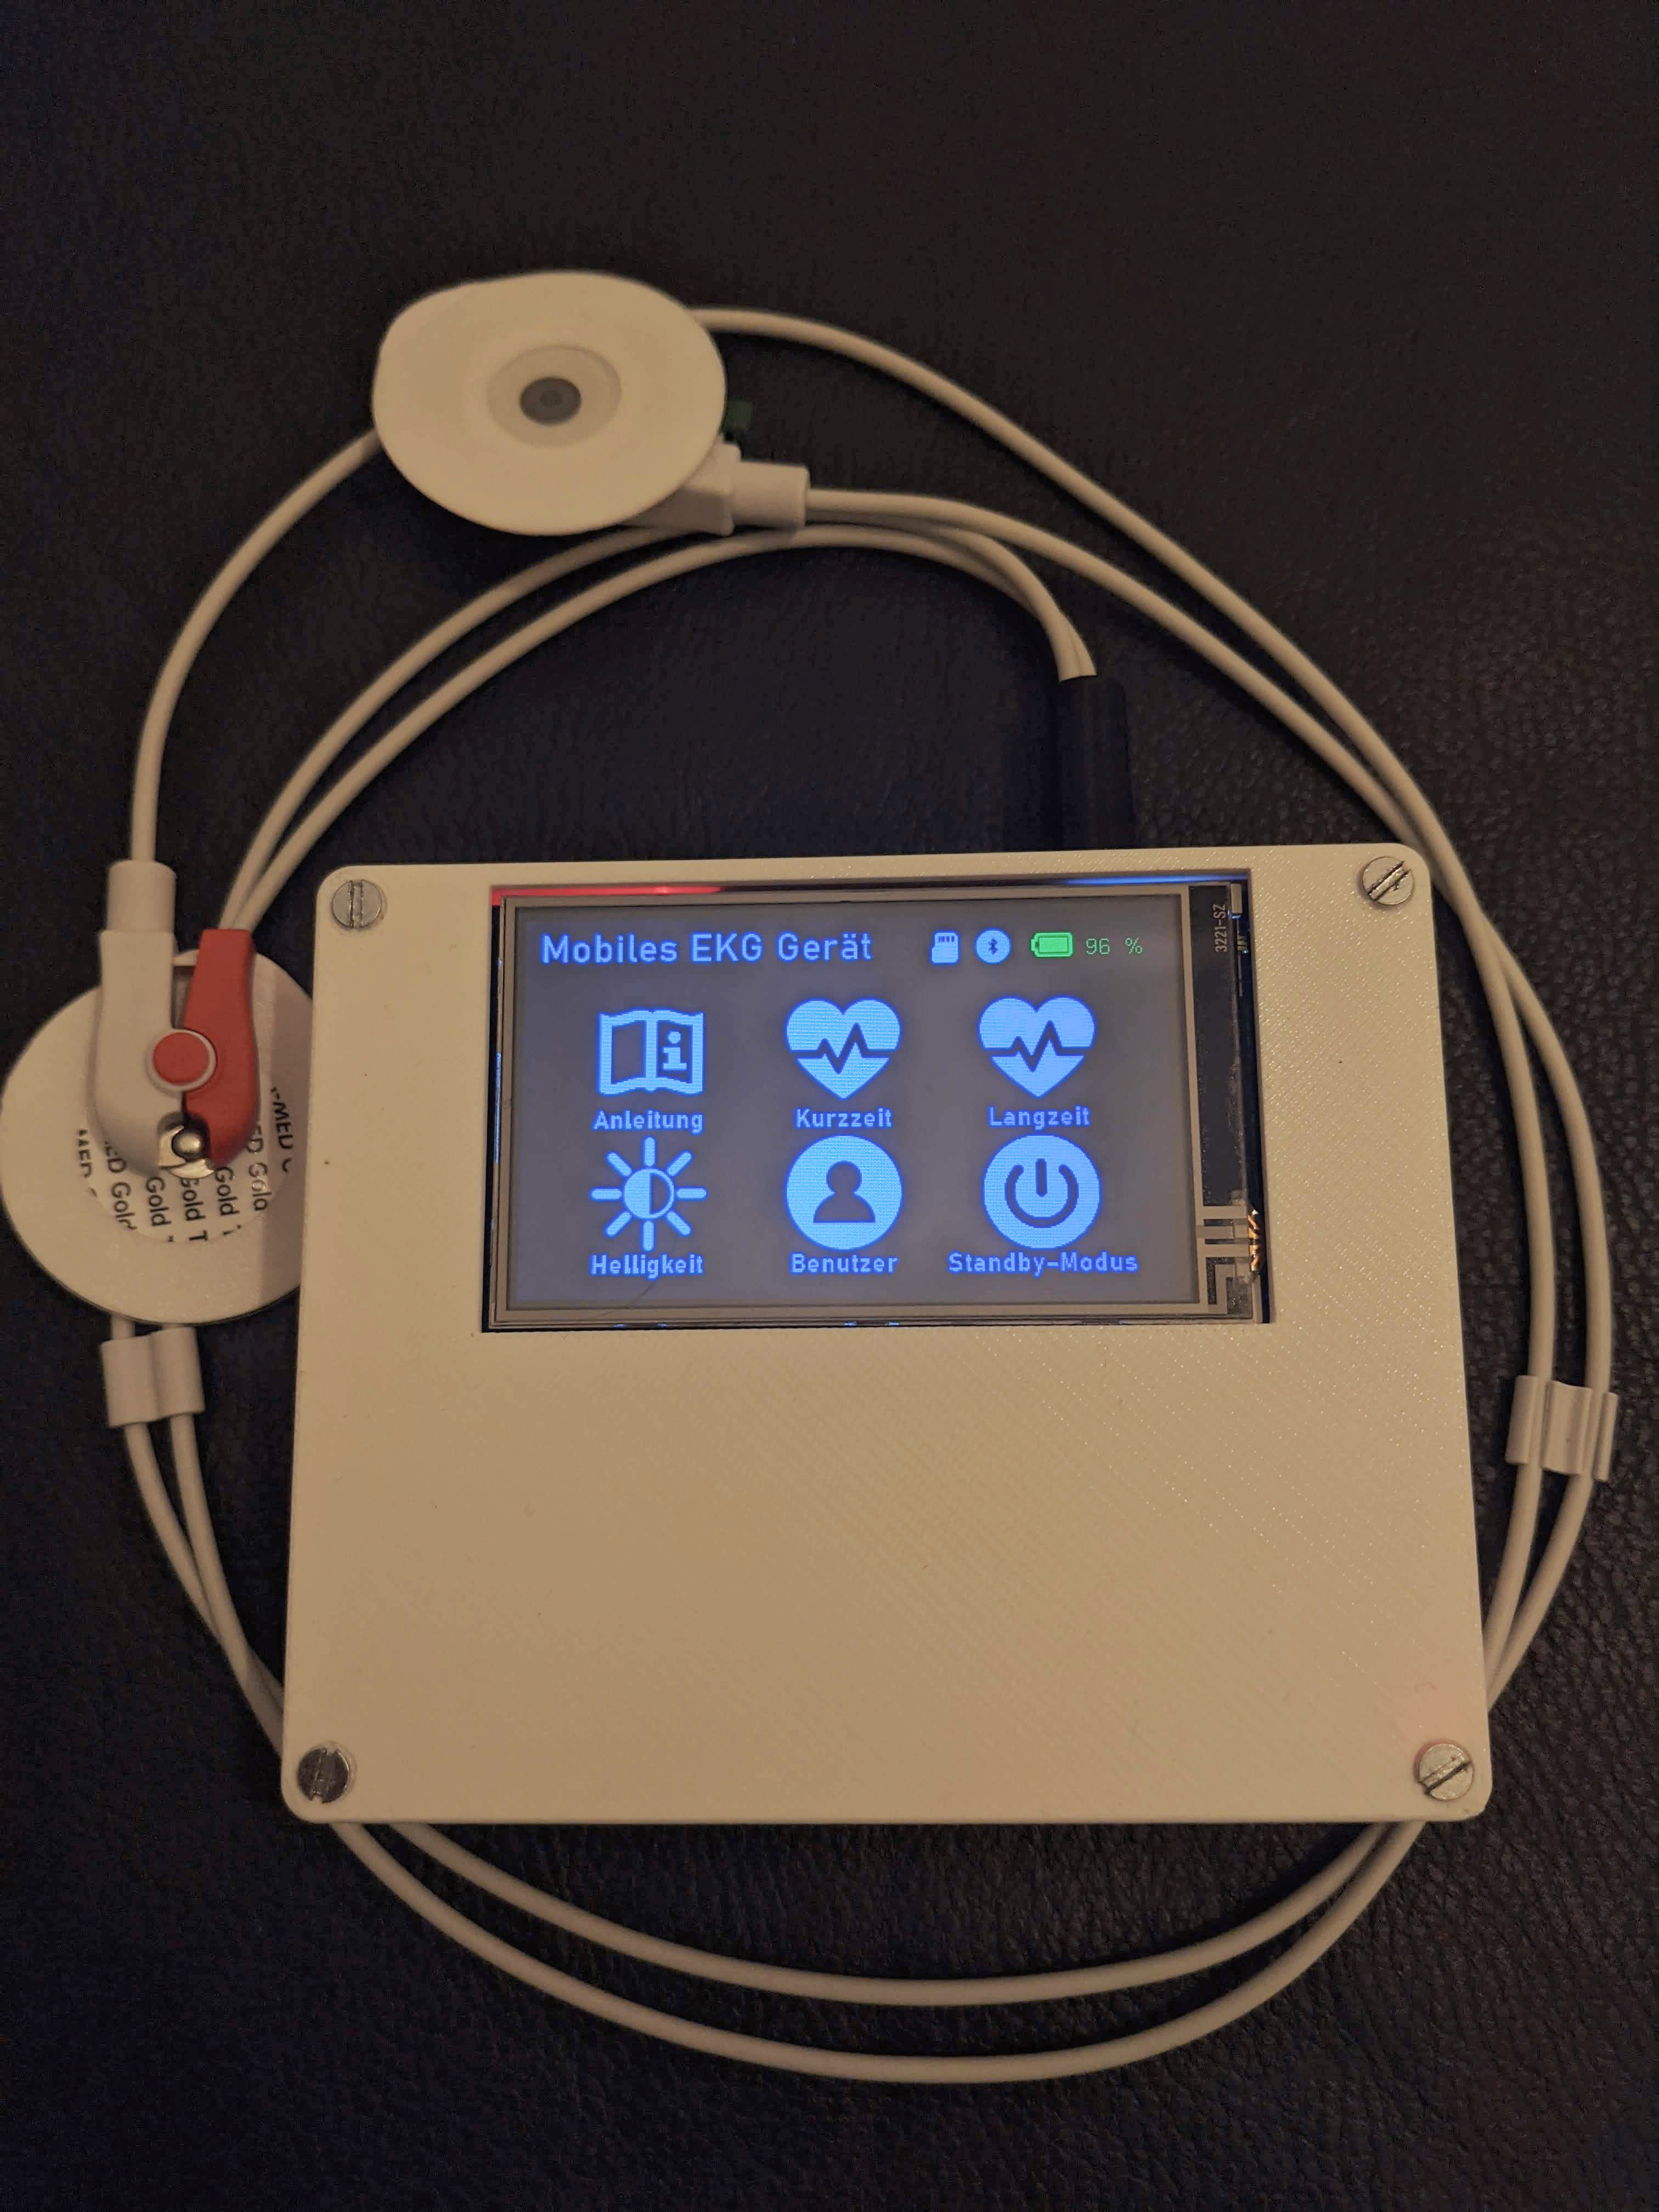
\includegraphics[width=\textwidth] {EKG_hell.jpg}
	\caption{Fertiges EKG-Gerät}
	\label{fig_EKG-Gerät} 
\end{figure}

\subsection{Ausblick/ Verbesserungen}

Während der Entwicklung wurden mögliche Verbesserungen und Erweiterungen des aktuellen Projekts aufgeworfen, die Thema dieses Unterkapitels sind.

\begin{enumerate}

\item Zur Vereinfachung der Bedienung kann die Ladeschaltung des Akkus im Gehäuse integriert werden. So kann der Benutzer auch während des Ladevorgangs das Gerät nutzen.

\item Im aktuellen Stand des Projektes liegen das Bluetooth- und SD-Karten-Modul als separate Platinen vor, die über Flachbandkabel mit der Hauptplatine verbunden werden. Die Integration dieser Baugruppen auf der Hauptplatine, würde die Störanfälligkeit der Verkabelung eliminieren und das Gehäuse könnte noch kompakter entworfen werden.

\item Um den Energiesparmodus zu vereinfachen und allgemein mehr Freiheit bei der Verwaltung der einzelnen peripheren Module zu haben, würde es sich anbieten diese separat mit Strom zu versorgen. Hierfür bieten sich Feldeffekttransistoren an, die über das GPIO-Modul des Prozessors gesteuert angesteuert werden und die Energieversorgung der Peripherie zu- oder abschalten.

\item Um die Funktionalität zu erweitern, könnte wie bereits an anderen Stelle erwähnt, ein Algorithmus zur automatisierten Diagnose von Vorhofflimmern implementiert werden. Hierfür müsste ermittelt werden ob die Rechenleistung des MSP430 bei gleichbleibender Abtastrate ausreicht, oder ob externe Leistung (z.b. Smartphone, PC) nötig ist.

\item Aktuell dient die Android-App hauptsächlich zur Anzeige des Signals. Durch eine gegenseitige Kommunikation zwischen Smartphone und EKG-Gerät könnten die Bedienmöglichkeiten des Smartphones zur Steuerung des EKG genutzt werden. Beispielsweise könnte die Tastatur eines mobilen Devices genutzt werden um die Benutzerauswahl zu erweitern und detaillierte Patientendaten auf dem EKG-Gerät zu hinterlegen.

\item Mit einem größeren integrierten Display könnten Steuerungsmöglichkeiten zur Skalierung des Signals auf dem Display implementiert werden. In der aktuellen Version wurde darauf verzichtet, da die Auswahlfelder für die eindeutige Bedienung mit dem Finger eine Mindestgröße besitzen müssen.

\end{enumerate}